\documentclass{article}
\usepackage{graphicx}
\usepackage[margin=1.5cm]{geometry}
\usepackage{amsmath}

\begin{document}

\title{Tuesday Reading Assessment: Unit 4, Reactance and Impedance}
\author{Prof. Jordan C. Hanson}

\maketitle

\section{Memory Bank}

\begin{itemize}
\item $X_{\rm C} = 1/(2\pi f C)$ ... The reactance of a capacitor with capacitance $C$, at frequency $f$.
\item $X_{\rm L} = 2\pi f L$ ... The reactance of an inductor with inductance $L$, at frequency $f$.
\item $Z_{\rm tot} = \sqrt{R^2 + (X_{\rm L} - X_{\rm C})^2}$ ... The total impedance of a series circuit with resistance $R$, and reactances $X_{\rm C}$ and $X_{\rm L}$.
\item $\tau = RC$ ... The time constant of an RC circuit.
\item $f_0 = \frac{1}{2\pi\sqrt{LC}}$ ... The resonance frequency of an RLC circuit.
\end{itemize}

\section{Reactance, Impedance, and Waveforms}

\begin{figure}
\centering
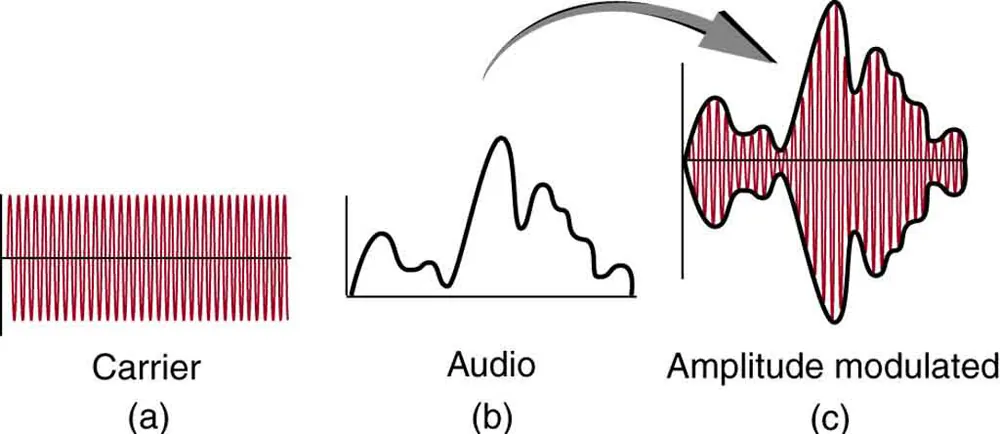
\includegraphics[width=0.55\textwidth]{figures/AM.png}
\caption{\label{fig:1} An example of an amplitude modulated (AM) waveform.}
\end{figure}

\begin{enumerate}
\item (a) What is the reactance of a capacitor with $C = 0.1$ $\mu$F at a frequency $f = 1$ MHz? (b) What will the reactance be at $f = 0.5$ MHz? (c) If this capacitor is installed in an RC circuit with a $50\Omega$ resistor, what is the total impedance? (d) What is the time constant of this circuit? \\ \vspace{1.5cm}
\item (a) What is the total impedance of an RLC circuit at $f = 10$ kHz, if $R = 100$ $\Omega$, and $C = 10$ pF, and $L = 1$ $\mu$H? (b) What is the resonance frequency of this circuit? \\ \vspace{1.5cm}
\item An amplitude modulated radio wave is generated by a mixer based on an LC resonating circuit (see Fig. \ref{fig:1}).  The carrier, with frequency $f_{\rm C}$, and the audio, with frequency $f_{\rm A}$, are \textit{mixed}.  The modulated result is comprised of two frequencies: $f_{\rm C} - f_{\rm A}$, and $f_{\rm C} + f_{\rm A}$. (a) If we have an audio signal at 4 kHz and a carrier at 1 MHz, what are the final frequencies? (b) Given what you know about \textit{filtering}, how would you construct a circuit that only responds to the signal at $f_{\rm C} + f_{\rm A}$?
\end{enumerate}
\end{document}
